% chercher des documents LaTeX dans styles, corps et bib
\makeatletter\def\input@path{{styles/}{corps/}{bib/}}\makeatother


\documentclass[12pt, openany]{report}
\usepackage[a4paper,vdivide={*,22cm,4cm}]{geometry}
\usepackage[french]{babel}
\selectlanguage{french}
\usepackage[T1]{fontenc}
\usepackage[utf8]{inputenc}
\usepackage{pageGardeEnsta}
\usepackage{lmodern}
\usepackage{enumitem}
\usepackage{subcaption}
\usepackage{hyperref}
% pour charger des images
\usepackage{graphicx}
% répertoire dans lequel trouver les images
\graphicspath{{imgs/}}
% liens hypertexte dans le document
\usepackage[colorlinks,breaklinks]{hyperref}
\setlength{\parindent}{0pt}
\usepackage{float}
\usepackage{hyperref}
\usepackage{listings}
\usepackage[round]{natbib}

\title{Véhicule autonome \\ suiveur de lignes}
\author{Colin Baumgard, Ludovic Diguet, Hamid Hacene, Corentin Lemoine, Antonin Lizé}
\date{\today}
\doctype{Middleware}
\promo{UE 4.1}
\etablissement{\textsc{Ensta} Bretagne\\2, rue François Verny\\
  29806 \textsc{Brest} cedex\\\textsc{France}\\Tel +33 (0)2 98 34 88 00\\ \url{www.ensta-bretagne.fr}}
\logoEcole{\includegraphics[height=4.2cm]{logo_ENSTA_Bretagne_Vertical_CMJN}}
\imgGarde{\centering\includegraphics[scale=0.4]{result.png}}

\renewcommand{\thesection}{\arabic{section}}
\begin{document}
\maketitle
\tableofcontents
\pagebreak

\section*{Introduction}
\addcontentsline{toc}{chapter}{Introduction}
Ce projet s'inscrit dans le cadre des enseignements de l'\textsc{ENSTA Bretagne} dispensés aux élèves de deuxième année de la filière \textit{Robotique Autonome} au sein de l'U.E 4.1 : \textit{Middleware}.\\

Sed sed porttitor risus. Curabitur elit erat, aliquet non orci et, lacinia egestas libero. Suspendisse tristique diam eu efficitur tincidunt. Praesent rhoncus venenatis sapien, nec efficitur elit mattis et. Duis nec felis convallis nulla semper gravida a sit amet magna. Ut enim sapien, vehicula vel ultricies quis, pharetra vitae nunc. In hac habitasse platea dictumst.\\

Lorem ipsum dolor sit amet, consectetur adipiscing elit. Pellentesque ac diam vulputate, dictum turpis ac, mattis ligula. Maecenas ornare, metus a fringilla vestibulum, leo ex pellentesque magna, vel lobortis elit est ac magna. Mauris porta consequat lorem, quis tristique mauris porttitor sed. Nam quam ipsum, placerat vitae mi sed, mattis accumsan tortor.\\

\section*{Abstract}
\addcontentsline{toc}{chapter}{Abstract}
Lorem ipsum dolor sit amet, consectetur adipiscing elit. Pellentesque ac diam vulputate, dictum turpis ac, mattis ligula. Maecenas ornare, metus a fringilla vestibulum, leo ex pellentesque magna, vel lobortis elit est ac magna. Mauris porta consequat lorem, quis tristique mauris porttitor sed. Nam quam ipsum, placerat vitae mi sed, mattis accumsan tortor.\\

Sed sed porttitor risus. Curabitur elit erat, aliquet non orci et, lacinia egestas libero. Suspendisse tristique diam eu efficitur tincidunt. Praesent rhoncus venenatis sapien, nec efficitur elit mattis et. Duis nec felis convallis nulla semper gravida a sit amet magna. Ut enim sapien, vehicula vel ultricies quis, pharetra vitae nunc. In hac habitasse platea dictumst.

\pagebreak

\section{Présentation du projet}
\subsection{Problématique}
Nous avons pu acquérir au fil du semestre quatre une connaissance théorique et pratique du \textit{Middleware} \textsc{ROS} (Robot Operating System). Pour rappel, un \textit{Middleware} est un outil qui permet d'échanger des informations entre différentes applications et programmes via des techniques et des messages standardisés. \textsc{ROS} est un \textit{Middleware} développé par l'\textsc{Open Robotics}.\\

Le but de ce projet au sein de l'U.E est de maîtriser les concepts fondamentaux de \textsc{ROS} et d'arriver à les implémenter sur un robot. Il s'agit d'appliquer une démarche d'ingénierie afin de proposer des solutions adéquates en prenant en compte les différentes dimensions techniques du problème : \textit{hardware} et \textit{software}.\\

La problématique de départ se résume ainsi à "rendre un véhicule autonome pour accomplir un tour complet du terrain d'athlétisme de l'école". Les véhicules mis à disposition sont des voitures à l'échelle $1/10^ème$ construite par différents groupes au semestre précédent.

\begin{figure}[!h]
     \centering
     \begin{subfigure}[b]{0.45\textwidth}
         \centering
         \includegraphics[width=\textwidth, height = 5cm]{terrain.jpg}
         \caption{Terrain de l'\textit{ENSTA Bretagne}}
     \end{subfigure}
     ~
     \begin{subfigure}[b]{0.45\textwidth}
         \centering
         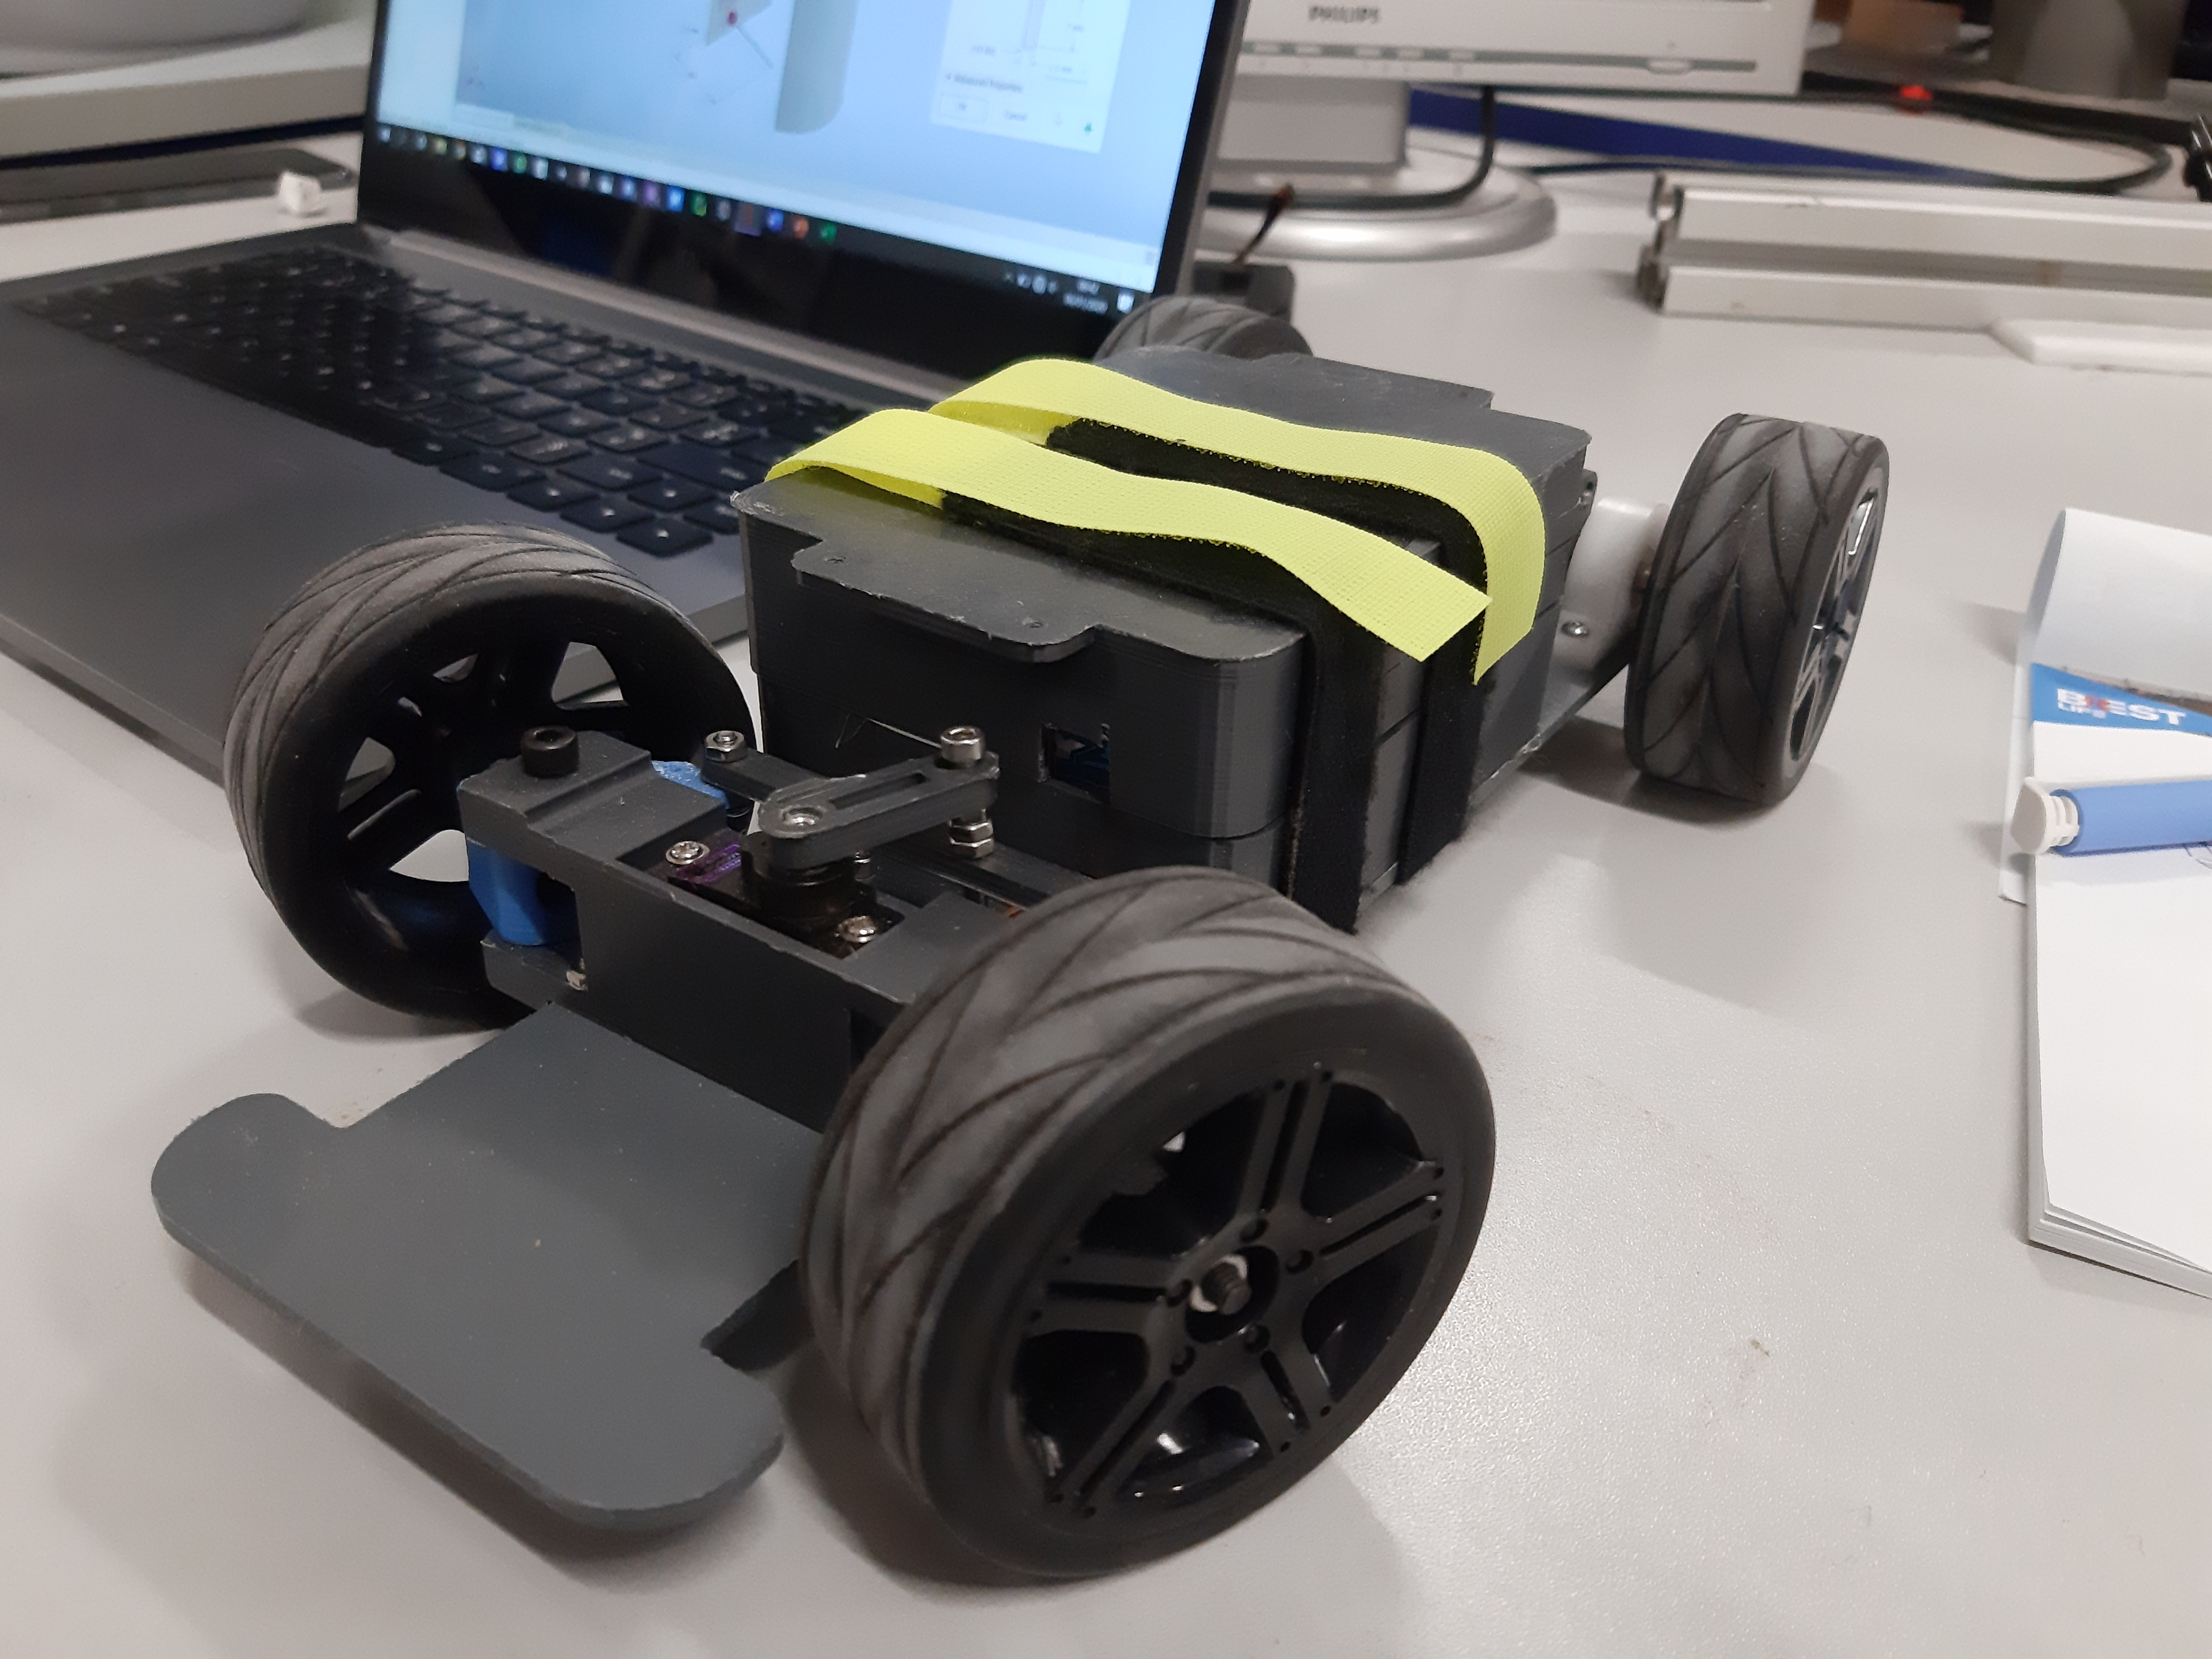
\includegraphics[width=\textwidth, height = 5cm]{voiture.jpg}
         \caption{Voiture utilisée pour le projet}
     \end{subfigure}
     \caption{Problématique du projet}
     \label{fig:prob}
\end{figure}

\subsection{Objectifs}
L'objectif principal de notre équipe est de répondre à la problématique tout en proposant une approche différente des autres groupes pour apporter une diversité aux contenus des projets.\\

Ainsi, nous nous sommes fixé ces deux objectifs supplémentaires : 
\begin{itemize}[label=\textbullet, font=\small]
    \item Proposer une approche réaliste qui s'inspire des voitures autonomes existantes sur le marché ou en développement ;
    \item Développer essentiellement en \textsc{C++} pour garantir la portabilité des algorithmes et l'implémentation sur d'autres structures ;\\
    \item Utiliser le plus possible les solutions et algorithmes proposés par \textsc{ROS} afin d'exploiter au maximum les possibilités offertes par ce \textit{Middleware}.\\
\end{itemize}

Compte tenue de l'évolution de la pandémie du \textit{Covid-19}, et suite à la fermeture de l'\textit{ENSTA Bretagne}, nous avons revu la problématique et les objectifs du projets. À cause d'une avarie de matériel, l'objectif principal ne peut être atteint : il s'agit désormais de construire une simulation pour valider les différents algorithmes qui seront proposés.

\section{Support matériel}
\subsection{Présentation de la voiture}
Sed sed porttitor risus. Curabitur elit erat, aliquet non orci et, lacinia egestas libero. Suspendisse tristique diam eu efficitur tincidunt. Praesent rhoncus venenatis sapien, nec efficitur elit mattis et. Duis nec felis convallis nulla semper gravida a sit amet magna. Ut enim sapien, vehicula vel ultricies quis, pharetra vitae nunc. In hac habitasse platea dictumst.\\

--> Expliquer vite fait la construction de la voiture + photo + schéma

\subsection{Adaptation de l'architecture pour le projet}
Sed sed porttitor risus. Curabitur elit erat, aliquet non orci et, lacinia egestas libero. Suspendisse tristique diam eu efficitur tincidunt. Praesent rhoncus venenatis sapien, nec efficitur elit mattis et. Duis nec felis convallis nulla semper gravida a sit amet magna. Ut enim sapien, vehicula vel ultricies quis, pharetra vitae nunc. In hac habitasse platea dictumst.\\

--> Citer les sensors qui équiperont la voiture !\\

--> Expliquer tous les changements apportés à la voiture de base : pièces supplémentaires (support caméra, support Rasp, batterie, support GPS, etc...) avec schéma et pk ces choix techniques de conception !

\section{Simulation sous \textsc{V-REP}}
\subsection{Modélisation dynamique de la voiture}
Sed sed porttitor risus. Curabitur elit erat, aliquet non orci et, lacinia egestas libero. Suspendisse tristique diam eu efficitur tincidunt. Praesent rhoncus venenatis sapien, nec efficitur elit mattis et. Duis nec felis convallis nulla semper gravida a sit amet magna. Ut enim sapien, vehicula vel ultricies quis, pharetra vitae nunc. In hac habitasse platea dictumst.\\

--> Expliquer vite fait la modélisation de la voiture en faisant référence au tp de Benn Zerr.

\subsection{Création de la piste}
Sed sed porttitor risus. Curabitur elit erat, aliquet non orci et, lacinia egestas libero. Suspendisse tristique diam eu efficitur tincidunt. Praesent rhoncus venenatis sapien, nec efficitur elit mattis et. Duis nec felis convallis nulla semper gravida a sit amet magna. Ut enim sapien, vehicula vel ultricies quis, pharetra vitae nunc. In hac habitasse platea dictumst.\\

--> Expliquer comment la piste a été construite et surtout justifier le choix de la texture (vraie route !)

\subsection{Interface avec \textsc{ROS}}
Sed sed porttitor risus. Curabitur elit erat, aliquet non orci et, lacinia egestas libero. Suspendisse tristique diam eu efficitur tincidunt. Praesent rhoncus venenatis sapien, nec efficitur elit mattis et. Duis nec felis convallis nulla semper gravida a sit amet magna. Ut enim sapien, vehicula vel ultricies quis, pharetra vitae nunc. In hac habitasse platea dictumst.\\

--> Mettre les équation d'états de la voiture et expliquer quels sont les variables à contrôler\\

--> Expliquer l'interface avec ROS : lua pour la caméra et le control de steering + speed\\

--> Maintenant comment rendre cette voiture autonome ?!

\section{Choix techniques}
\subsection{Architecture fonctionnelle}
Sed sed porttitor risus. Curabitur elit erat, aliquet non orci et, lacinia egestas libero. Suspendisse tristique diam eu efficitur tincidunt. Praesent rhoncus venenatis sapien, nec efficitur elit mattis et. Duis nec felis convallis nulla semper gravida a sit amet magna. Ut enim sapien, vehicula vel ultricies quis, pharetra vitae nunc. In hac habitasse platea dictumst.\\

--> Mettre l'arch fct.\\

--> Expliquer les différentes briques : GPS, PWM, etc..

\section{Pipeline de contrôle}
\subsection{Architecture \textit{C2}}
Sed sed porttitor risus. Curabitur elit erat, aliquet non orci et, lacinia egestas libero. Suspendisse tristique diam eu efficitur tincidunt. Praesent rhoncus venenatis sapien, nec efficitur elit mattis et. Duis nec felis convallis nulla semper gravida a sit amet magna. Ut enim sapien, vehicula vel ultricies quis, pharetra vitae nunc. In hac habitasse platea dictumst.\\

--> Mettre l'arch C2 (node graphe ??) et expliquer les grandes étapes.

\subsection{Window Lane Detection}
Sed sed porttitor risus. Curabitur elit erat, aliquet non orci et, lacinia egestas libero. Suspendisse tristique diam eu efficitur tincidunt. Praesent rhoncus venenatis sapien, nec efficitur elit mattis et. Duis nec felis convallis nulla semper gravida a sit amet magna. Ut enim sapien, vehicula vel ultricies quis, pharetra vitae nunc. In hac habitasse platea dictumst.\\

--> Expliquer toute la pipeline de traitement d'image en détaillant les fonctions et montrer les résultats intermédiaires !

\section{Résultats}
Sed sed porttitor risus. Curabitur elit erat, aliquet non orci et, lacinia egestas libero. Suspendisse tristique diam eu efficitur tincidunt. Praesent rhoncus venenatis sapien, nec efficitur elit mattis et. Duis nec felis convallis nulla semper gravida a sit amet magna. Ut enim sapien, vehicula vel ultricies quis, pharetra vitae nunc. In hac habitasse platea dictumst.\\

--> Mettre les résultats obtenues + lien vers vidéo !

\section{Perspectives et améliorations}
--> Mettre toutes les améliorations possibles (Docker)

\section*{Conclusion}
\addcontentsline{toc}{chapter}{Conclusion}
Lorem ipsum dolor sit amet
coming Soon !!

\section*{Annexe1 : Raspberry comme ordinateur de bord}
\addcontentsline{toc}{chapter}{Annexe1}

Nous avons choisi d'installer Raspbian sur notre raspberry, cela nous permet d'avoir un accès simple à la caméra, cependant l'installation de ROS est un peu plus longue, car il faut recompiler les sources.

Pour installer ROS sur notre raspberry pi 3 nous avons suivi la documentation officielle :  \url{http://wiki.ros.org/ROSberryPi/Installing%20ROS%20Kinetic%20on%20the%20Raspberry%20Pi}



\section*{Annexe2 : Installation des librairies}
\addcontentsline{toc}{chapter}{Annexe2}
Lorem ipsum dolor sit amet
coming Soon !!

\end{document}